\setchapterimage[6cm]{cabecera2}
\setchapterpreamble[u]{\margintoc}
%%%%%%%%%%%%%%%%%%%%%%%%%%%%%%%%%%%%%%%%%%%%%%%%%%%%%%%%%%%%%

\chapter{Replicación}
\label{ch:Replicaci\'on}
\index{replicación}


\section{Replicaci\'on}

Una de las razones para usar la t\'ecnica de replicación es  aumentar la disponibilidad de servicios.
Si algunos datos se almacenan exclusivamente en un solo nodo y ese nodo deja de funcionar, ya no se podrá acceder a los datos. Pero si los datos se replican en su lugar, los clientes pueden cambiar sin problemas a una réplica.

 Factores que son relevantes para la alta disponibilidad  son la ocurrencia de fallas en los  servidores y las particiones de red con  desconexi\'on de operaciones  (no planificadas y pueden ser un efecto secundario de la movilidad del usuario).
 
 Las particiones de red dificultan la construcción de detectores de fallas,
 que se utilizan para lograr una multidifusión confiable y totalmente ordenada.
  

 Otra razón para la replicación es aumentar la escalabilidad y el rendimiento; Cuantas más réplicas haya, más clientes podrán acceder a los datos simultáneamente sin sufrir degradaciones de rendimiento. 
  \sidecite{Gorton2022}  \sidecite{Fekete2010} \sidecite{Helal1996}

No obstante, la replicaci\'on de datos debe asegurar que   los clientes  no deben tener en cuenta que existen múltiples copias físicas de datos, quiere decir esto que debe haber  transparencia en la replicación. 
Los datos se organizan como objetos lógicos individuales e identifican solo un elemento en cada caso cuando solicitan que se realice una operación. Se 
 espera que las operaciones devuelvan solo un conjunto de valores. 

Las operaciones se realizan sobre una colección de objetos replicados produce resultados que cumplen con la especificación de corrección para esos objetos, es decir, se asegura la  consistencia de datos.

Sin embargo, en una  operación que ha sufrido de desconexi\'on se puede permitir que los datos se vuelvan inconsistentes, temporalmente. Pero cuando los clientes permanecen conectado,  no es aceptable que diferentes clientes (con diferentes copias físicas de datos) obtengan resultados inconsistentes cuando las solicitudes afectan  el mismos objetos lógicos.  
 
 \subsection{Administrador de Réplicas}
 \index{administradores de réplicas}
 Los Administradores de Réplicas son servidores cuya funcionalidad es la gestión de réplicas de objetos   

 En los  modelos de  administradores de réplicas  los componentes arquitectónicos se describen por sus roles y no se especifica la implementación (hardware). Puede aplicarse en un entorno cliente-servidor, (administrador de réplica es un servidor) o se puede aplicar a una aplicación y los procesos de la aplicación (servidores multiprocesos).  Ejemplo: computadora portátil del usuario   puede contener una aplicación que actúa como un administrador de réplicas para su sitio web.
 Se asume que cada administrador de réplicas mantiene una réplica de cada objeto 
 
 Los modelo administradores  de réplicas:
 \begin{itemize}
 	\item  aplica operaciones a sus réplicas de forma recuperable ( una operación en un administrador de réplicas no deja resultados inconsistentes si ocurren fallas) 
 	\item  Un administrador de réplicas puede ser una máquina de estado    \sidecite{Lamport1978} \sidecite{Schneider1990} Las operaciones en sus réplicas equivale a realizar operaciones en una secuencia estricta. Es decir, el estado de sus réplicas es una función determinista de sus estados iniciales y la secuencia de operaciones que les aplica)
	 \item 	Se asume que el administrador de réplicas mantiene una réplica de cada objeto. Sin embargo, las réplicas de diferentes objetos pueden ser mantenido por diferentes conjuntos de administradores de réplica. 
 	\item El conjunto de administradores de réplica puede ser estático o dinámico. En un sistema dinámico, pueden aparecer nuevos administradores de réplica (por ejemplo, si una segunda persona  copia un sitio web en su computadora portátil).
 		
 \end{itemize}


En la figura \ref{fig:adm-rep} se muestra un modelo de arquitectura para el administrador de datos replicados: una colección de administrador de réplicas ofrece un servicio a los clientes. Los clientes  solicitan una serie  operaciones o invocaciones sobre  los objetos.  Las operaciones solicitadas son de solo lectura. o actualización. 
 Las solicitudes de  cliente son manejadas primero por el front-end (FE)
 El rol del FE es comunicarse mediante un mensaje que pasa a los  administrador de réplicas.
 FE es el  vehículo para hacer el modelo transparente la replicación.
 Se puede implementar un FE en la dirección del espacio del cliente, o puede ser un proceso separado 
 
  \begin{figure}%
 	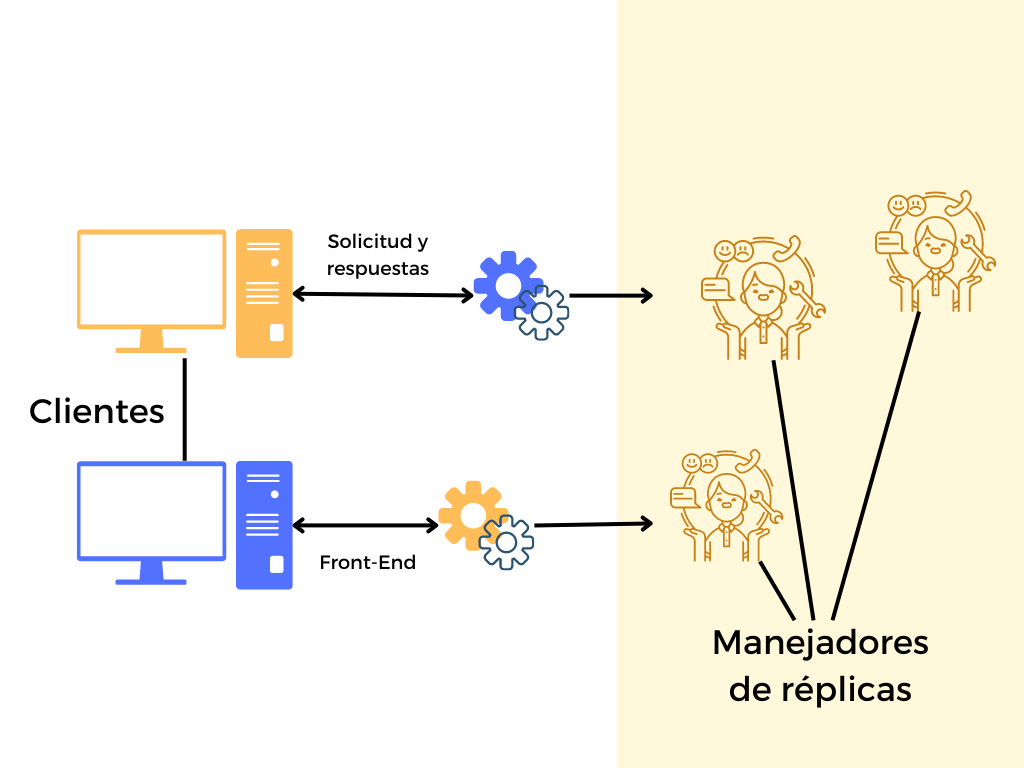
\includegraphics {9/4.png } 
 	\caption{Arquitectura del administrador de replicas de datos}
 	\label{fig:adm-rep}
 \end{figure}
 
  
 
 Un protocolo de replicaci\'on  \sidecite{Pedone2000}, ver figura  \ref{fig:protocol-sol}, es un modelo abstracto que sirve como base para describir los modelos de replicaci\'on. Este protocolo  se describe en una secuencia de cinco pasos. :

  \index{protocolo de replicación}
 
  \begin{enumerate} 	
 	\item Solicitud:   FE emite la solicitud a uno o más administradores de réplica:
		\begin{itemize}
			\item FE se comunica con un solo administrador de réplica.
			\item o FE  difunde usando multidifusi\'on ,la solicitud al resto de 	administradores de réplica.
		\end{itemize} 
 	\item  	Coordinación: administrador de réplica se coordinan para ejecutar la solicitud  de manera consistente.
 	Acuerda, si  la solicitud se aplica o decide sobre la misma.  El orden de los mensajes pueden ser:
 	\begin{itemize}
 		\item FIFO: si un FE emite la solicitud  $r$  antes que la solicitud $r'$, los  administradores de réplica  maneja  $r'$ despues de resolver $r$.  
 		\item Orden causal: si  $r \rightarrow r '$ , los administradores de réplica  resuelven   $r$ antes de  que $r'$ .
 		\item Orden total: administrador de réplica maneja $r$  antes de la solicitud  $r'$ , entonces otro administrador de réplica  maneja $r'$  despues  de  $r$ .
 	\end{itemize} 	
 	
 	\item Ejecución: administrador de réplica ejecutan la solicitud, de  manera que puedan deshacer sus efectos más tarde. 
 	\begin{itemize}
 		\item 	Acuerdo: los administrador de réplica llegan a consenso sobre el efecto de la solicitud, si la hay,  se compromete.  
 		\item Respuesta: Uno o más administrador de réplica responden al FE. 
 		Un administrador de réplica envía la respuesta. 
 		O FE recibe respuestas de una colección de administrador de réplica y selecciona o una respuesta única a pasar al cliente. 
 		
 	\end{itemize} 
 \end{enumerate}


   
 
 \begin{figure}%
 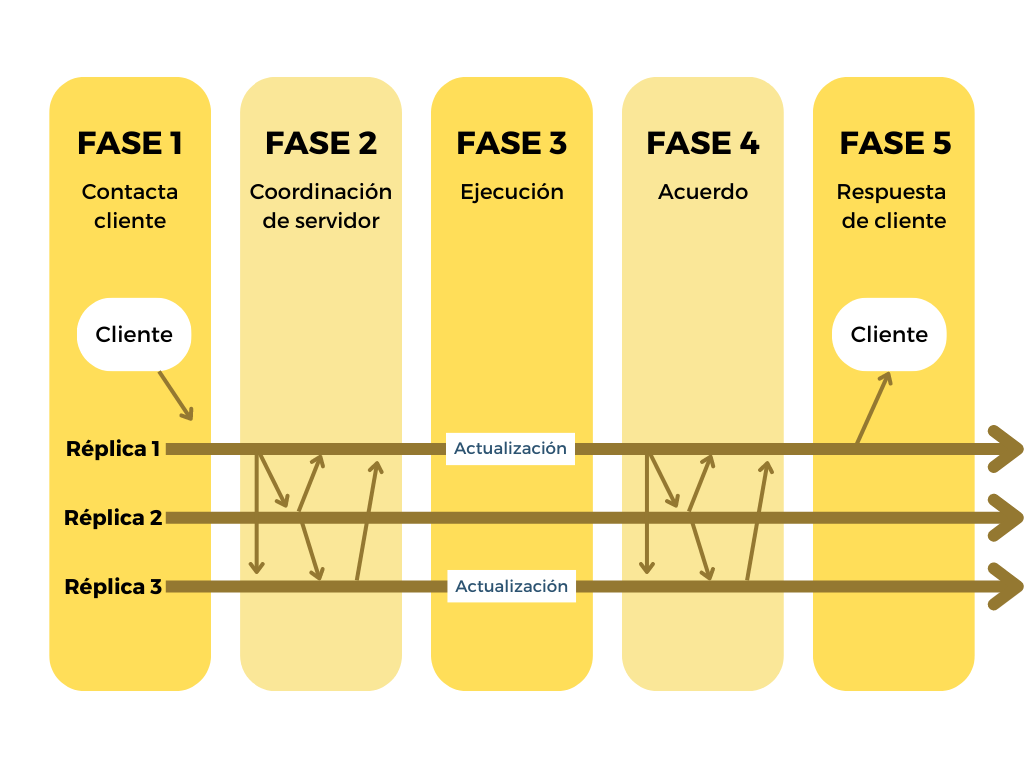
\includegraphics {9/3.png} 
 \caption{Protocolo de una solicitud. Tomado de \cite{Pedone2000}}
 \label{fig:protocol-sol}
 \end{figure}
 
 \section{Tolerancia a Fallas}
   \index{tolerancia a fallas}
   
   Los servicios tolerantes a fallos son aquellos servicios que ante la  presencia de fallos cumplen la especificación  o responde correctamente.
   Obtener respuesta suele ser parte de la especificación (disponibilidad).
   Por su repetición, los fallos pueden ser:   transitorios,  intermitentes o permanentes.
   En cuanto a los fallos, aquellos relacionados con procesos ( ver en tabla \ref{tab:cat-middle} en cap\'itulo \ref{cap:def-SD}, estos se pueden clasificar de acuerdo a su  tipo en:  fallos de bloqueo,   fallos de parada o  fallas bizantinas
   
   
   Para construir servicios tolerantes a fallos se basa en ofrecer redundancia en:
   \begin{itemize}
   	\item De información (datos replicados, códigos redundantes, CRC).
   	 \item Temporal (retransmisiones, repetición de transacciones abortadas).
   	 \item Física (componentes, máquinas, conexiones replicados).
   	  \item De información y física combinadas (discos espejo, RAID).
   \end{itemize}
   
   La redundancia puede introducir a su vez fallos (respuestas incorrectas) en los servicios. Entonces, ¿Cómo proporcionar un servicio que sea correcto a pesar de la ocurrencia de fallas en el proceso?
   
   
   
 Existen varios criterios de corrección para objetos replicados. Algunos de estos  criterios de consistencia son la  Linealizabilidad,  Consistencia secuencial y  Consistencias débiles.
 
 \subsection{Linealizabilidad y Consistencia Secuencial}
 \paragraph{Linealizabilidad}
  \index{linealizabilidad}
  Los sistemas más estrictamente correctos son linealizables y esta propiedad se denomina linealizabilidad (\textit{linearizability}). 
 
 La linealizabilidad es la forma más fuerte de \gls{consistencia}. Esto significa que todas las operaciones se ejecutan como si se ejecutaran en una sola máquina, a pesar de que los datos se distribuyen en múltiples réplicas. Como resultado, cada operación devuelve un valor actualizado.
 
 Un servicio de objetos compartidos replicados es linealizable si para cualquier ejecución existe algún entrelazamiento de las series de operaciones emprendidas por cada cliente que satisfaga:
 \begin{itemize}
 	\item  La secuencia entrelazada de operaciones cumple la especificación de una (única) copia correcta de los objetos.
 	\item El orden de las operaciones del entrelazamiento es consistente con los tiempos reales en los cuales ocurrieron las operaciones en la ejecución real.
 \end{itemize}
 
 \paragraph{Ejemplo de Linealizibilidad }
 
 
 En el siguiente ejemplo de la figura \ref{fig:ejm-lin}, es el esquema de procesos en un  sistema distribuido con tres procesos diferentes: $P_{1}$, $P_{2}$ y $P_{3}$. El cliente $A$ escribe un valor 1 en un objeto $A$. Dado que el sistema es linealizable, una vez que se completa la operación de escritura, todas las lecturas posteriores deben devolver el valor de esa escritura o el valor de la operación de escritura posterior. 
 
 Entonces, cuando el cliente $B$ lee el valor de $A$, el resultado es $1$. Una vez que una operación de lectura devuelve un valor particular, todas las lecturas posteriores deben devolver ese valor o el valor de la operación de escritura posterior.
 
 
 \begin{figure}%
 	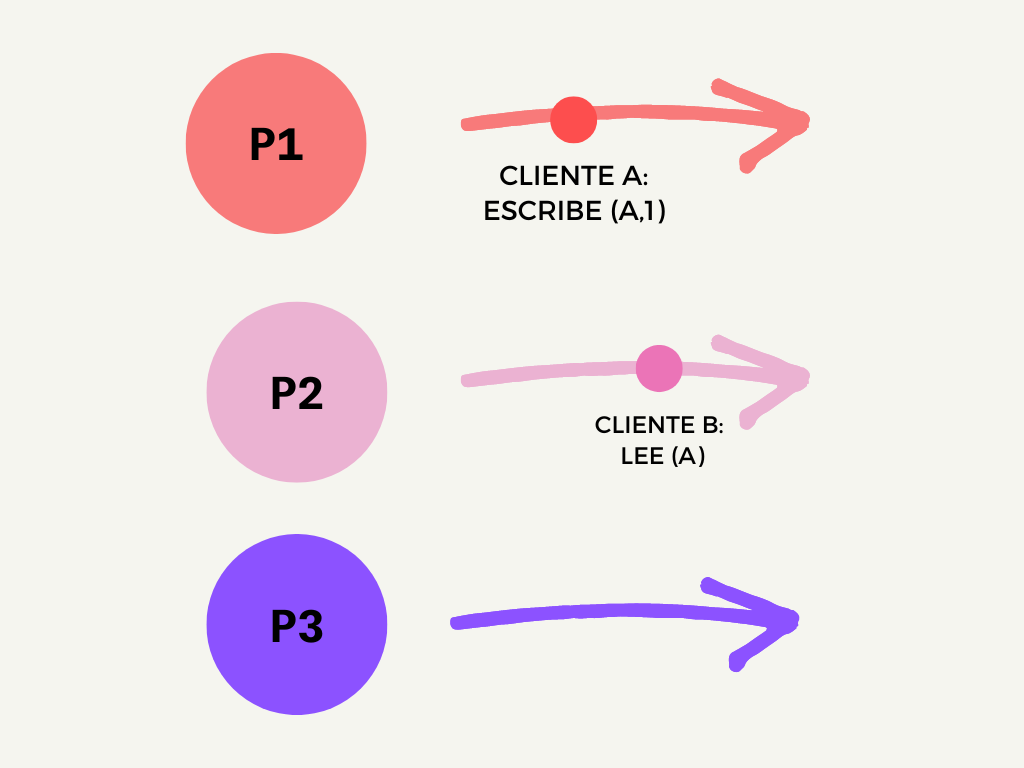
\includegraphics {9/1.png } 
 	\caption{Ejemplo de Linealizibilidad}
 	\label{fig:ejm-lin}
 \end{figure}
 

 \paragraph{ Consistencia secuencial} 
  \index{consistencia secuencial}
 
 La consistencia secuencial es una fuerte propiedad de seguridad para los sistemas concurrentes.  Se define \sidecite{Lamport1979} como el resultado de cualquier ejecución es el mismo que si las operaciones de todos los procesadores se ejecutaran en algún orden secuencial, y las operaciones de cada procesador individual aparecen en esta secuencia en el orden especificado por su programa.
 
 
 Un servicio es consistente secuencialmente si para alguna
 de las posibles secuencias de operaciones intercaladas:
 \begin{itemize}
 	\item El orden de las operaciones en el intercalado es consistente con
 	el orden de programa que ejecuta cada cliente individual
 	 \item Dicho orden en serie ‘real’ es consistente con las copias u
 	operaciones realizadas
 	 \item Cualquier servicio linealizable es consistente
 	secuencialmente, pues el orden real de ejecución refleja el
 	orden del programa.  Lo contrario no es cierto 
 \end{itemize}
 
 
 El resultado de cualquier ejecución es el mismo que si las operaciones (lectura y escritura) de todos los procesos en el almacén de datos fueron ejecutados en algún orden secuencial y las operaciones de cada proceso individual aparecen en esta secuencia en el orden especificado por su programa. 
 
 
  Existen varios modelos o técnicas de replicación tolerantes a fallas. A continuaci\'on se presentan dos de ellas:
 
 
 \subsection{Modelo de Replicación Pasiva}
  \index{replicación pasiva}
 
 En el modelo de replicación pasiva \sidecite{Pedone2000} , tambi\'en  modelo de replicación de Respaldo Primario con tolerancia a fallas, ver figura \ref{fig:rep-pas}, el modelo tiene un único administrador de réplica  primarias y uno o más administrador de réplica secundarios, tambi\'en nominados como  copias de seguridad o esclavos. 
 FE se comunican solo con el administrador de réplica principal para obtener el servicio. El administrador de réplica principal ejecuta las operaciones y envía copias de los datos actualizados a copias de seguridad 
 Si el primario falla, una de las copias de seguridad se modifica para actuar como el primario.
 
 La secuencia de eventos cuando un cliente solicita que se realice una operación:
 
 \begin{itemize}
 	\item  Solicitud: FE emite la solicitud, que contiene un ID único, al administrador de réplica principal. 
 	\item Coordinación: el servidor primario toma cada solicitud atómicamente, en el orden de su recepción. Comprueba el ID único, en caso de que ya haya ejecutado la solicitud, y si es así,  reenvía la respuesta. 
 	\item Ejecución: el servidor primario ejecuta la solicitud y almacena la respuesta.
  	
 	\item Acuerdo: si la solicitud es una actualización, el servidor primario envía el estado actualizado, la respuesta y el ID único a todas las copias de seguridad. Las copias de seguridad envían un acuse de recibo. 
 	\item Respuesta: El servidor primario responde al FE, que devuelve la respuesta al cliente.
 \end{itemize}

 
 El sistema implementa la linealización si el servidor primario es correcto, el servidor  primario secuencia  las operaciones sobre los objetos compartidos. 
 Si el servidor primario falla, entonces el sistema conserva la capacidad de linealización si una única copia de seguridad se convierte en el nuevo servidor primario y si la nueva configuración del sistema toma el control exactamente donde quedó el último.
 El servidor primario se reemplaza por una copia de seguridad. 
 Los administrador de réplica sobrevivientes acuerdan qué operaciones se realizaron en el momento en que se hace cargo el reemplazo del servidor  primario.
 
 
 	\begin{figure}%
 		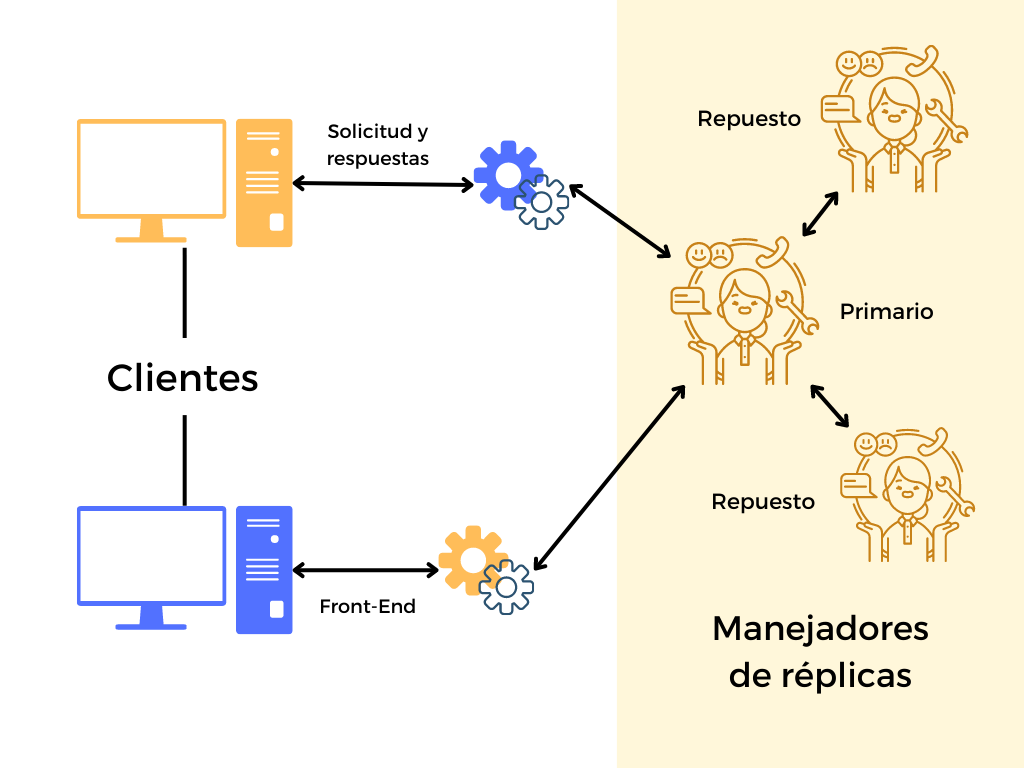
\includegraphics {9/5.png} 
 		\caption{Modelo de Replicación Pasiva. Adaptado de \cite{Coulouris2011}}
 		\label{fig:rep-pas}
 	\end{figure}
 
  \subsection{Modelo de Replicación Activa} 	
	   \index{replicación activa}
 
	
	 En los modelos de  replicación activa \sidecite{Coulouris2011}, los administradores de réplica son máquinas de estado que juegan roles equivalentes y están organizados como un grupo. 
	La figura \ref{fig:rep-act} se plasma la  arquitectura del modelo de  replicación activa. Los servidores FE distribuyen sus solicitudes al grupo de administrador de réplica y todos  procesan la solicitud de forma independiente pero idéntica y responden a cada una de ellas. 
	 Si un administrador de réplica falla, esto no afecta el rendimiento del servicio, ya que los administradores de réplica restantes continúan respondiendo de la manera normal. 
	Este modelo es  tolerarnte a las  fallas bizantinas, porque el FE puede recopilar y comparar las respuestas que recibe.
	 
	 La secuencia de  operación en el modelo:
	 \begin{itemize}
	 	\item  Solicitud: el FE adjunta un ID único a la solicitud y lo transmite al grupo de administrador de réplica, utilizando una primitiva de multidifusión confiable y totalmente ordenada. 
	 	Se supone que si el FE falla al estrellarse en el peor de los casos. No emite la siguiente solicitud hasta que recibe una respuesta. 
	 	\item Coordinación: el sistema de comunicación grupal entrega la solicitud a cada administrador de réplica correcto en el mismo orden (total) 
	 	
	 	\item Ejecución: cada administrador de réplica ejecuta la solicitud. Como son máquinas de estado y las solicitudes se entregan en el mismo orden total, los AR correctos procesan la solicitud de manera idéntica. La respuesta contiene el  ID de solicitud del cliente. 
	 	\item Acuerdo: no se necesita una fase de acuerdo, debido a la semántica de entrega de multidifusión. 
	 	\item Respuesta: Cada administrador de réplica envía su respuesta al FE. El número de respuestas que recopila el FE depende de los supuestos de falla y el algoritmo de multidifusión 
	 \end{itemize}
	 
 \begin{figure}%
 	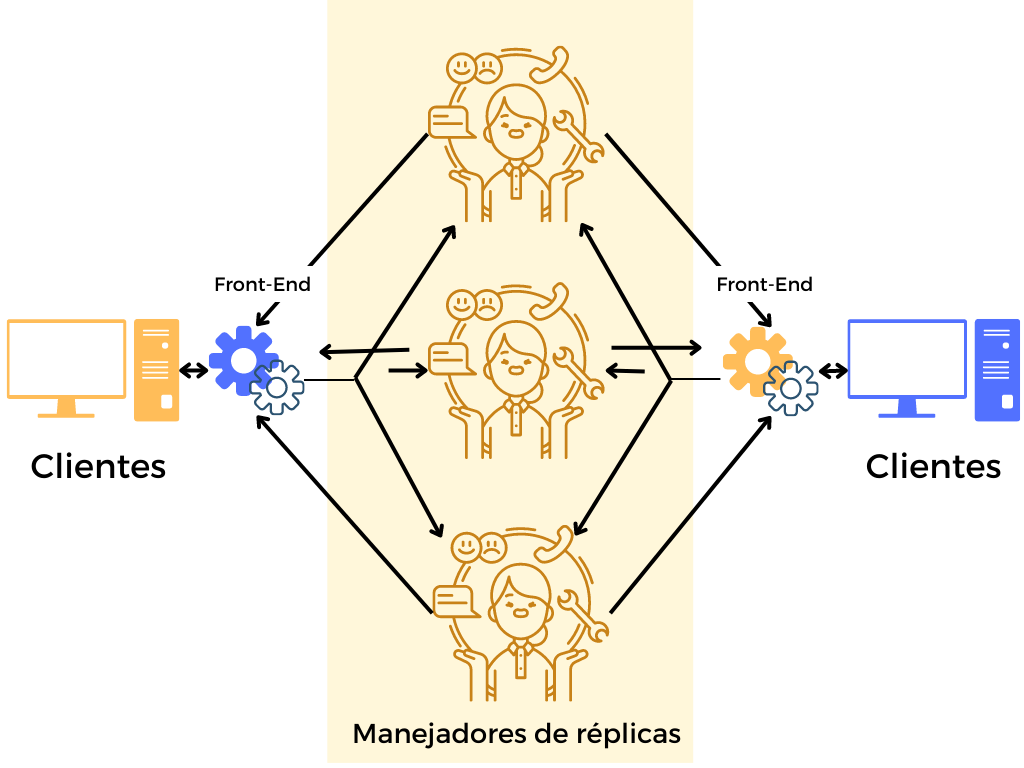
\includegraphics {9/2.png } 
 	\caption{Modelo de Arquitectura de Replicación Activa. Adaptado de \cite{Coulouris2011} }
 	\label{fig:rep-act}
 \end{figure}
 
 El modelo de replicaci\'on activa logra consistencia secuencial:
 \begin{itemize}
 	\item Todos los administrador de réplica  procesan la misma secuencia de solicitudes. La confiabilidad de la multidifusión asegura que cada administrador de réplica  procese el mismo conjunto de solicitudes y el orden total asegura que las procesen en el mismo orden.
 	\item  	Como son máquinas de estado, todas terminan con el mismo estado que las demás después de cada solicitud. Las solicitudes de cada FE se atienden en Orden FIFO (FE espera una respuesta antes de hacer la siguiente solicitud).
 	\item Si los clientes no se comunican con otros clientes mientras esperan respuestas a sus solicitudes, entonces sus solicitudes se procesan en el orden anterior.  
 	\item Por otra parte, si los clientes son multiproceso y pueden comunicarse entre sí mientras esperan respuestas del servicio. Para garantizar el procesamiento de la solicitud en el orden anterior, tendríamos que reemplazar la multidifusión por una que esté causal y totalmente ordenada. 
 	\item El sistema de replicación activa no logra linealización. Esto se debe a que el orden total en el que los administradores de réplicas procesan las solicitudes no es necesariamente el mismo que el orden en tiempo real en el que los clientes hicieron sus solicitudes.
 \end{itemize}
 
 \section{Caso de Estudio. Fragmentación}
  \index{caso de estudio!cache} \index{caso de estudio!fragmentación}
  
 La \gls{fragmentacion}  \sidecite{Saino2016} es una técnica ampliamente utilizada para escalar horizontalmente  sistemas de almacenamiento y caché, y abordar los cuellos de botella en la capacidad de procesamiento y almacenamiento. Según esta técnica, un gran conjunto de elementos se divide en un conjunto de segmentos, denominados fragmentos,  de acuerdo  al resultado de una función hash calculada en  el identificador del objeto. Luego, cada fragmento se asigna a un dispositivo de almacenamiento físico o de caché. 
 
 La fragmentación es un patrón de arquitectura de base de datos \sidecite{Ozsu2020} que divide una única base de datos en tablas más pequeñas conocidas como fragmentos, cada una almacenada en un nodo independiente. Cada partición de base de datos se conoce como fragmento lógico y su almacenamiento dentro de un nodo se conoce como fragmento físico.
 Esta técnica  permite dividir datos entre los miembros de un clúster e identificar el miembro del clúster responsable de un elemento determinado simplemente calculando una función hash. La fragmentación se usa ampliamente en una variedad de aplicaciones como  en sistemas de bases de datos, cachés web en redes empresariale  y almacenes  clave-valor.  
 
 
\subsubsection{?`Fragmentación, partición o replicación?}
 
  ¿Cuál es la diferencia entre fragmentación y partición? Fragmentación, partición y replicación son conceptos similares, pero con diferencias importantes entre ellos. De hecho, la fragmentación puede considerarse una clase especial de partición.
 
 El particionamiento se define como cualquier división de una base de datos en partes distintas, generalmente por motivos como un mejor rendimiento y facilidad de gestión \sidecite{Ozsu2020}  \sidecite{Harrison2016}. Dependiendo de la situación, se puede utilizar particiones horizontales o verticales:
 
 \begin{itemize}
 	\item   Partición horizontal: cada partición utiliza el mismo esquema de base de datos y tiene las mismas columnas, pero contiene filas diferentes.
 	\item Partición vertical: cada partición es un subconjunto adecuado del esquema de base de datos original, es decir, contiene todas las filas, pero solo un subconjunto de las columnas originales.
 	
 \end{itemize}

 La fragmentación suele ser un caso de partición horizontal. Existen varios esquemas de fragmentación posibles para determinar cómo particionar los datos en una base de datos:
 \begin{itemize}
 	\item Fragmentación basada en rango: la base de datos se fragmenta en función de un valor determinado, como el nombre o el número de identificación. Por ejemplo, una base de datos de estudiantes universitarios puede fragmentarse según la primera letra de su apellido.
 	\item  Fragmentación basada en hash: esta técnica se utiliza para bases de datos clave-valor. La clave de cada entrada de la base de datos se pasa a través de una función hash, que genera un resultado que determina a qué fragmento se asignará la entrada.
 \end{itemize}
 
Un ejemplo de una base de datos fragmentada se muestra en la Figura \ref{fig:fragmen}.
 
 	\begin{figure}%
 	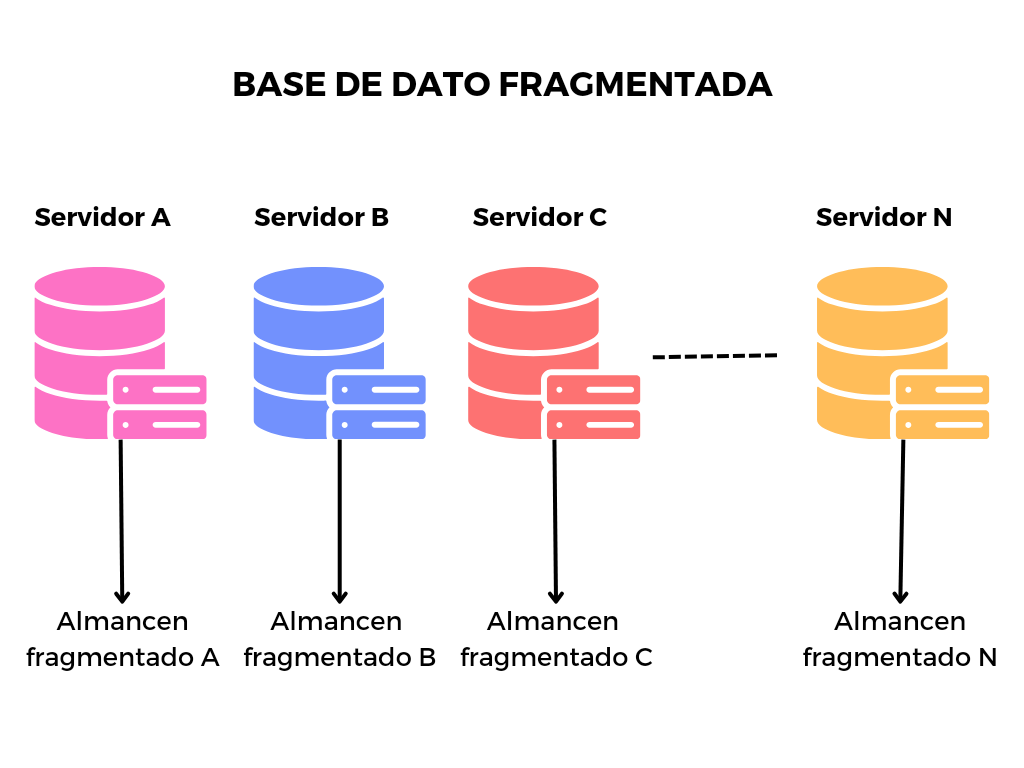
\includegraphics {9/6.png} 
 	\caption{Fragmentaci\'on de base de datos}
 	\label{fig:fragmen}
 \end{figure}
 
 Mientras la replicación  es el   término de  hacer una copia  de la información de una base de datos en otra ubicación. La fragmentación y la replicación son estrategias separadas, pero complementarias, para mejorar la disponibilidad de la base de datos.  
 
 \subsubsection{Almacenamiento en  caché fragmentado}
 \index{caché fragmentado}
 
 Como ejemplo de  un sistema fragmentado, esta sección proporciona una presentaci\'on  diseño de un sistema de almacenamiento en caché fragmentado. Un caché fragmentado  \cite{Burns2018} es un almacenamiento  caché que se encuentra entre las solicitudes del usuario y la implementación real del frontend. En la Figura 6-2 se muestra un diagrama de alto nivel del sistema. En la Figura \ref{fig:fragmen-cache} se muestra la arquitectura de un cache fragmentado.
 
 
 
 \begin{figure}%
 	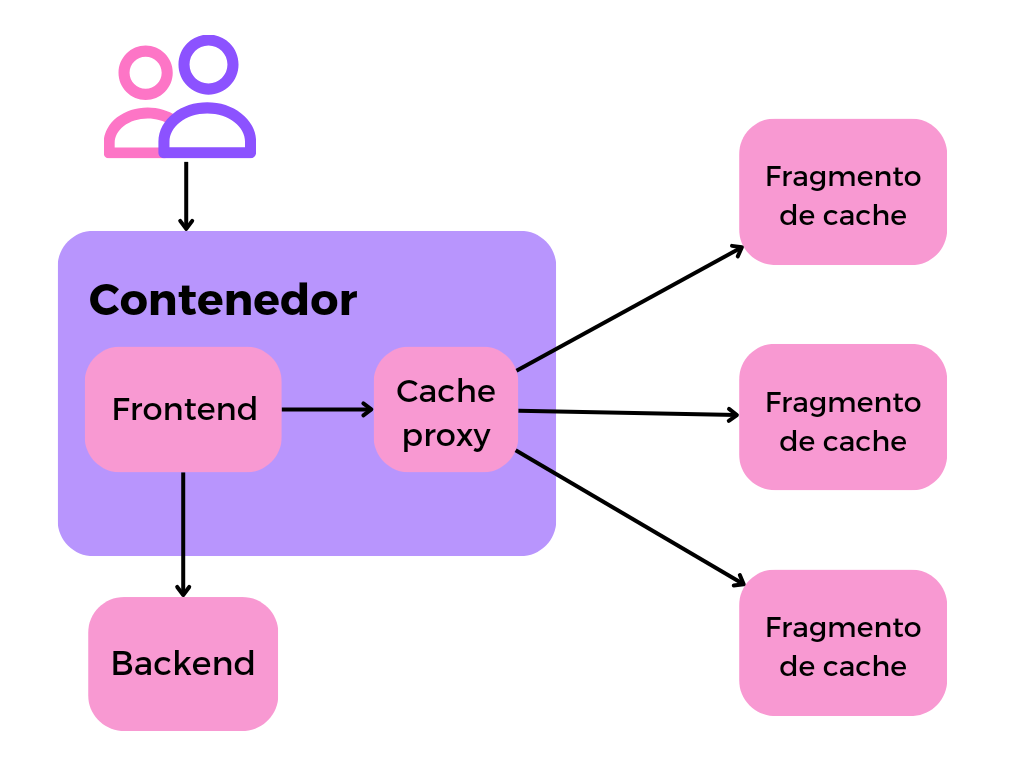
\includegraphics {9/7.png} 
 	\caption{Fragmentaci\'on de datos}
 	\label{fig:fragmen-cache}
 \end{figure}
  
  \paragraph{?` Por qu\'e se necesita fragmentar el caché ?}
  La razón principal para fragmentar cualquier servicio es aumentar el tamaño de los datos que se almacenan en el servicio.
   Para comprender cómo ayuda esto a un sistema de almacenamiento en caché, imagine el siguiente sistema \cite{Burns2018}: cada caché tiene 10 GB de RAM disponibles para almacenar resultados y puede atender 100 solicitudes por segundo (RPS). Supongamos   que nuestro servicio tiene un total de 200 GB de resultados posibles que podrían devolverse y un RPS esperado de 1000. Esto puede implementarse mediante  replicaci\'on con  10 réplicas del caché para satisfacer 1000 RPS (10 réplicas × 100 solicitudes por segundo por réplica). Esta implementaci\'on contendr\'ia  un máximo del $5\%$    (10 GB/200 GB) del conjunto de datos total que estamos sirviendo. 
   Usando un caché   fragmentado de 10 vías, aún podemos servir la cantidad adecuada de RPS (10 × 100 sigue siendo 1000), pero debido a que cada caché sirve un conjunto de datos completamente único, podemos aumentar el almacenamiento al $50\% $ ( 10 × 10 GB/200 GB) del conjunto de datos total. 
   
   \paragraph{Beneficios de utilizar caché fragmentado }
   
    A continuación se detallan algunos de sus beneficios:
    
    \begin{itemize}
    	\item  Uso de caché más eficiente. Sólo se necesita una copia de un archivo para todos los servidores de los centros de datos. 
    	\item Reduce la carga en el servidor de origen. Los servidores de una red de dsitribuci\'on de contenido utilizan la clave hash para determinar si hay contenido en la caché del grupo. El origen solo se solicita si el grupo no tiene ningún contenido almacenado en caché. Esto reduce los costos en los que se incurre al pagar por el tráfico desde los servidores de la red hasta el origen. 
    	\item Velocidad de entrega de contenido mejorada. Verificar las cachés de los servidores cercanos en un grupo en busca de un archivo es más rápido que enrutar una solicitud al origen. 
    	
    \end{itemize}
    
    \paragraph{Caché fragmentado y replicado}
    Un servicio fragmentado y replicado combina el patrón de servicio replicado  con el patrón fragmentado. En  lugar de que un único servidor implemente cada fragmento de la caché, se utiliza un servicio replicado para implementar cada fragmento de la caché. En la Figura \ref{fig:cache-frag-rep} se muestra un esquema de una base de datos de clientes fragmentada  por la inicial de su nombre. Cada fragmento tiene dos r\'eplicas. Note que esta distribuci\'on puede cambiar  de  acuerdo a las necesidades del usuario.
    
     
    \begin{figure}%
     	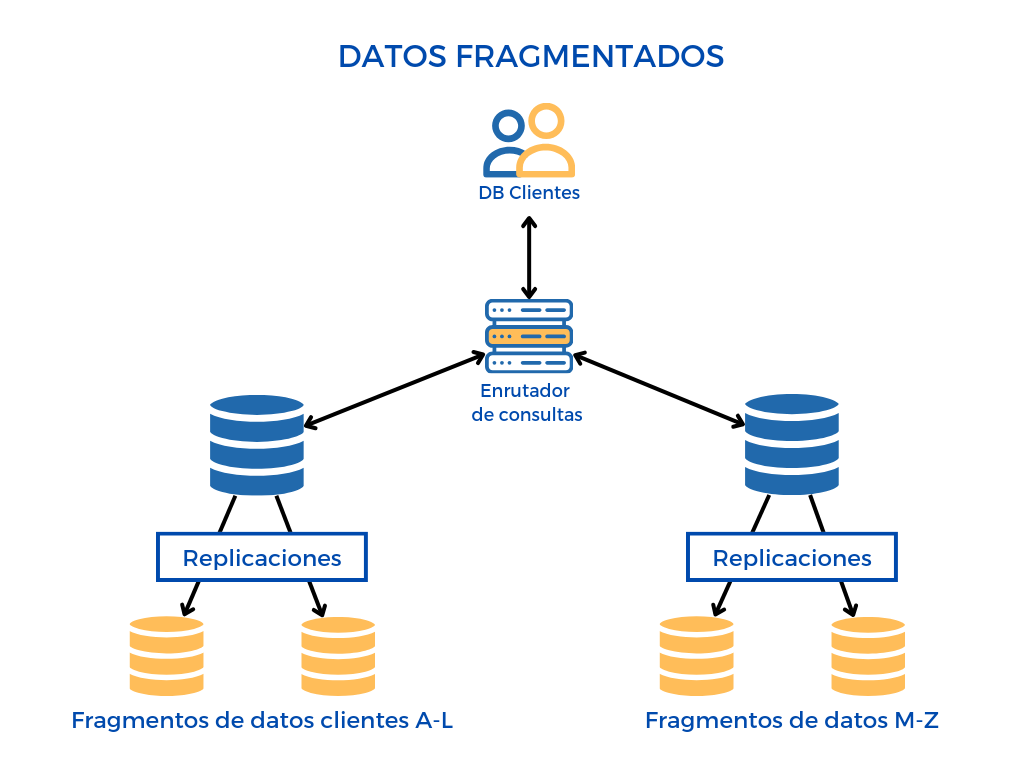
\includegraphics {9/8.png} 
    	\caption{Caché fragmentado y replicado }
    	\label{fig:cache-frag-rep}
    \end{figure}
   
   Este diseño es más complicado de implementar, pero tiene varias ventajas sobre un servicio fragmentado simple. Lo más importante es que, al reemplazar un único servidor con un servicio replicado, cada fragmento de caché es resistente a las fallas y siempre está presente durante la ocurrencia de  fallas. Adem\'as se espera una mejora del rendimiento que proporciona la memoria caché. 
   
  
  
  

 